\chapter{Ejercicio 2: DAXPY}

\section{Introducción}

    El algoritmo DAXPY (\textit{Double-precision Alpha X Plus Y}) constituye una operación fundamental en álgebra lineal que forma parte del conjunto estándar de rutinas BLAS (\textit{Basic Linear Algebra Subprograms}). Esta operación vectorial realiza la combinación lineal $y = \alpha x + y$, donde $x$ y $y$ son vectores de tamaño $n$ y $\alpha$ es un escalar. Su aparente simplicidad esconde una importancia capital en computación científica, ya que sirve como componente esencial en numerosos algoritmos más complejos como multiplicación de matrices, resolución de sistemas lineales, y cálculo de autovalores, entre otros.

    DAXPY se caracteriza por su alta intensidad de acceso a memoria combinada con operaciones aritméticas relativamente simples, lo que lo convierte en un excelente candidato para evaluar el rendimiento de los sistemas de memoria en arquitecturas paralelas. Esta relación entre operaciones de memoria y computación hace que el algoritmo esté típicamente limitado por el ancho de banda de memoria más que por la capacidad de cómputo, especialmente en plataformas de alto rendimiento como las GPUs modernas.
    
    Este apartado presenta una implementación optimizada de DAXPY utilizando CUDA con el paradigma de memoria unificada, analizando exhaustivamente su rendimiento en la GPU NVIDIA A100 disponible en el centro de supercomputación CESGA. Se examinará no solo el rendimiento bruto, sino también aspectos como la escalabilidad, eficiencia de utilización de recursos, y comparativas entre diferentes configuraciones para identificar las estrategias óptimas de implementación.

\newpage
    
\section{Fundamentos teóricos}

    \subsection{Algoritmo DAXPY}
    
        El algoritmo DAXPY (\textit{Double-precision Alpha X Plus Y}) realiza la siguiente operación matemática:
        
        \begin{align}
            y_i = \alpha \cdot x_i + y_i, \quad \text{para } i = 0, 1, \ldots, n-1
        \end{align}
    
        Donde:
        
        \begin{itemize}
        
            \item $x$ y $y$ son vectores de números en punto flotante de doble precisión.
            
            \item $\alpha$ es un escalar constante de doble precisión.
            
            \item $n$ es el tamaño de los vectores.
            
        \end{itemize}

        Esta operación vectorial, a pesar de su aparente simplicidad, es omnipresente en aplicaciones científicas y de ingeniería. Su importancia radica en que constituye un bloque fundamental para operaciones más complejas como productos escalares, multiplicación de matrices, resolución de sistemas de ecuaciones y algoritmos iterativos. En métodos numéricos, DAXPY aparece constantemente en técnicas como el descenso del gradiente, métodos de Krylov y factorizaciones matriciales.
        
        El algoritmo DAXPY se caracteriza por las siguientes propiedades computacionales:

        \begin{itemize}
        
            \item \textbf{Intensidad aritmética baja}: Una multiplicación y una suma por cada dos accesos a memoria (lectura de $x_i$ y lectura/escritura de $y_i$), lo que resulta en una ratio operaciones relativamente bajo. Esto convierte a DAXPY en un algoritmo típicamente limitado por el ancho de banda de memoria (\textit{memory-bound}).
            
            \item \textbf{Patrones de acceso regulares}: Los accesos secuenciales a memoria permiten optimizaciones como la precarga (\textit{prefetching}) y el uso efectivo de cachés, lo que es especialmente relevante en arquitecturas con jerarquías de memoria complejas.
            
            \item \textbf{Independencia de datos}: Cada elemento del vector se procesa independientemente de los demás, lo que permite una paralelización perfecta sin necesidad de sincronización entre hilos. Esta característica hace que DAXPY sea intrínsecamente paralelizable.
            
            \item \textbf{Localidad espacial}: Los accesos contiguos a memoria favorecen mecanismos de \textit{hardware} como la coalescencia en GPUs y vectorización en CPUs modernas.
            
        \end{itemize}

        La combinación de estas características hace que DAXPY sea no solo un componente crítico en computación científica, sino también un excelente \textit{benchmark} para evaluar el rendimiento de los subsistemas de memoria, la eficiencia de paralelización y la capacidad de aprovechamiento del \textit{hardware} en diferentes arquitecturas computacionales.

    \subsection{Memoria unificada en CUDA}
    
        La memoria unificada representa un avance significativo en el modelo de programación CUDA, introducida oficialmente en CUDA 6.0. Este paradigma proporciona un espacio de direcciones unificado accesible tanto desde la CPU como desde la GPU, abstrayendo la complejidad de la gestión explícita de transferencias de datos entre los diferentes espacios de memoria.
    
        Conceptualmente, la memoria unificada crea la ilusión de un espacio de memoria compartido mediante un sofisticado sistema de gestión de páginas a nivel del \textit{driver} y del \textit{hardware}. El runtime de CUDA, en colaboración con el sistema operativo, se encarga de:
    
        \begin{itemize}
        
            \item \textbf{Simplificación de la programación}: Elimina la necesidad de gestionar explícitamente las transferencias de memoria entre \textit{host} y \textit{device}, reduciendo significativamente la complejidad del código. Esto es particularmente valioso en algoritmos como DAXPY donde el patrón de acceso a datos es relativamente sencillo.

            \item \textbf{Gestión automática de páginas}: El sistema se encarga dinámicamente de mover las páginas de memoria entre CPU y GPU según sea necesario, implementando políticas de migración y replicación basadas en los patrones de acceso observados durante la ejecución.
            
            \item \textbf{Sobrecarga reducida}: Al minimizar la duplicación de datos entre diferentes espacios de memoria, se reduce el consumo total de memoria y se simplifican los patrones de comunicación entre \textit{host} y \textit{device}.
            
            \item \textbf{Coherencia automática}: El sistema mantiene la coherencia de los datos entre CPU y GPU, eliminando la necesidad de sincronización manual que sería necesaria con la gestión explícita de memoria.
            
        \end{itemize}
        
        A pesar de estas ventajas, la memoria unificada presenta consideraciones importantes que deben tenerse en cuenta:
        
        \begin{itemize}
        
            \item \textbf{Paginación bajo demanda}: La migración de páginas se produce cuando se accede a memoria no disponible localmente, lo que puede introducir latencias significativas si no se gestiona adecuadamente. Estas latencias pueden ser especialmente notables en el primer acceso a una región de memoria.
            
            \item \textbf{\textit{Overhead} de gestión}: El sistema de memoria virtual subyacente introduce cierta sobrecarga relacionada con la traducción de direcciones, gestión de fallos de página y migración de datos. En cargas de trabajo con patrones de acceso complejos o impredecibles, este \textit{overhead} puede ser considerable.
            
            \item \textbf{Rendimiento variable}: En algunos escenarios, particularmente con patrones de acceso irregulares o cuando el tamaño de los datos excede significativamente la memoria disponible en la GPU, el rendimiento puede ser inferior al de una gestión manual optimizada.
            
            \item \textbf{\textit{Prefetching} explícito}: Para maximizar el rendimiento, a menudo es necesario utilizar funciones como \texttt{cudaMemPrefetchAsync} para anticipar las necesidades de acceso y minimizar los fallos de página durante la ejecución crítica.
            
        \end{itemize}
    
        En el contexto específico del algoritmo DAXPY, la memoria unificada ofrece un equilibrio favorable entre simplicidad de implementación y rendimiento. Los patrones de acceso secuenciales y predecibles de DAXPY permiten que el sistema de gestión de memoria unificada anticipe eficientemente las necesidades de datos, mientras que la naturaleza intensiva en memoria del algoritmo se beneficia de la reducción en la duplicación de datos.
        
        Para volúmenes de datos extremadamente grandes, como los procesados en supercomputadoras como las disponibles en CESGA, las consideraciones de rendimiento relacionadas con la memoria unificada adquieren especial relevancia, ya que pueden influir significativamente en la escalabilidad y eficiencia global del algoritmo.

    \subsection{Configuración de bloques e hilos}

        La organización de los \textit{threads} en bloques y \textit{grids} constituye uno de los aspectos más críticos para el rendimiento en CUDA, ya que determina directamente cómo se mapea el paralelismo lógico del algoritmo a los recursos físicos disponibles en la GPU. En nuestra implementación, esta configuración se parametriza explícitamente, permitiendo un análisis sistemático de su impacto en el rendimiento:

        \begin{lstlisting}[language=C, caption={Calculo de dimensiones de bloques y \textit{grid}.}, gobble=12]
            int threadsPerBlock = atoi(argv[1]);
            long blocksPerGrid = ceil(n / threadsPerBlock);
        \end{lstlisting}

        Esta parametrización expone decisiones arquitectónicas fundamentales:
        
        \begin{enumerate}
        
            \item \textbf{Granularidad de los bloques}: El número de \textit{threads} por bloque determina la unidad básica de trabajo que se asigna a cada SM. Esta granularidad afecta múltiples aspectos del rendimiento:
            
                \begin{itemize}
                
                    \item \textbf{Utilización de recursos}: Cada bloque consume recursos específicos como registros y memoria compartida. Bloques más grandes pueden maximizar la utilización de estos recursos, pero podrían limitar el número de bloques concurrentes por SM.
                    
                    \item \textbf{Eficiencia de \textit{warps}}: Dado que los \textit{warps} son unidades de 32 \textit{threads}, tamaños de bloque que no sean múltiplos exactos de 32 resultarán en \textit{warps} parcialmente ocupados, desperdiciando capacidad computacional. Nuestra exploración sistemática incluye valores como 1, 2, 4, 8, 16, 32, 64, 128, 256, 512 y 1024 \textit{threads} por bloque, todos múltiplos exactos del tamaño de \textit{warp}.
                    
                    \item \textbf{Balanceo entre latencia y \textit{throughput}}: Bloques más pequeños permiten una granularidad más fina en la distribución del trabajo y potencialmente mayor solapamiento entre computación y acceso a memoria, mientras que bloques más grandes reducen el \textit{overhead} de gestión, pero pueden introducir desequilibrios en la carga de trabajo.
                    
                \end{itemize}
    
             \item \textbf{Dimensionamiento del \textit{grid}}: El número de bloques (\texttt{blocksPerGrid}) se calcula para cubrir completamente el espacio de datos, garantizando que cada elemento del vector sea procesado. Esta decisión tiene implicaciones arquitectónicas profundas:
                
                \begin{itemize}
                
                    \item \textbf{Escalabilidad}: Un número suficientemente grande de bloques asegura que todos los SMs disponibles reciban trabajo, maximizando la utilización global de la GPU. La fórmula utilizada garantiza que el número de bloques escale linealmente con el tamaño del problema.
                    
                    \item \textbf{Distribución dinámica}: El planificador de \textit{hardware} de la GPU distribuye los bloques entre los SMs disponibles de forma asíncrona. Un \textit{grid} con muchos bloques pequeños facilita un balanceo de carga más fino que uno con pocos bloques grandes.
                    
                    \item \textbf{\textit{Overhead} de planificación}: Cada lanzamiento y finalización de bloque implica cierto \textit{overhead}. Un número excesivo de bloques pequeños podría incrementar este \textit{overhead}, mientras que bloques demasiado grandes podrían causar desequilibrios en la fase final de ejecución.
                    
                \end{itemize}
            
        \end{enumerate}

        La influencia de estas decisiones de configuración se manifiesta directamente en métricas de rendimiento como la ocupancia efectiva, definida como la relación entre el número de \textit{warps} activos y el máximo teórico soportado por la arquitectura. En nuestra implementación, calculamos esta métrica utilizando la API de CUDA:
        
        \begin{lstlisting}[language=C, caption={Calculo de ocupancia teorica.}, gobble=12]
            int maxBlocksPerSM;
            cudaOccupancyMaxActiveBlocksPerMultiprocessor(&maxBlocksPerSM, daxpy, threadsPerBlock, 0);
            float occupancy = (float)(maxBlocksPerSM * threadsPerBlock / 32) /  (float)(prop.maxThreadsPerMultiProcessor / 32);
        \end{lstlisting}

        Este cálculo proporciona una estimación teórica de la eficiencia en la utilización de recursos, considerando factores como:

        \begin{itemize}
            
            \item \textbf{Registros por \textit{thread}}: Cada \textit{thread} en nuestro \textit{kernel} utiliza un número específico de registros determinado por el compilador de CUDA. Si este número es elevado, puede limitar la cantidad de \textit{warps} concurrentes por SM.
            
            \item \textbf{Memoria compartida por bloque}: Aunque nuestro \textit{kernel} no utiliza memoria compartida explícitamente, el sistema asigna cierta cantidad para variables temporales y comunicación intra-bloque.
            
            \item \textbf{Límites arquitectónicos}: La A100 tiene restricciones específicas como un máximo de 2048 \textit{threads} por SM, 1024 \textit{threads} por bloque, y 32 bloques por SM. Estas limitaciones establecen cotas superiores para la ocupancia alcanzable.
       
        \end{itemize}

        Es importante destacar que la ocupancia máxima no siempre se correlaciona directamente con el máximo rendimiento. En algoritmos \textit{memory-bound} como DAXPY, una ocupancia moderada puede ser suficiente para saturar el ancho de banda de memoria disponible, punto a partir del cual incrementos adicionales en la ocupancia producen beneficios marginales o incluso degradaciones de rendimiento por contención de recursos. Este comportamiento se analiza detalladamente en los resultados experimentales mediante la exploración sistemática de diferentes configuraciones de \textit{threads} por bloque.

    \subsection{Patrones de acceso a memoria}

        Los patrones de acceso a memoria constituyen uno de los factores más determinantes en el rendimiento de algoritmos ejecutados en GPU, especialmente para aquellos caracterizados como \textit{memory-bound} como es el caso de DAXPY. La arquitectura de memoria de la GPU está optimizada para patrones específicos de acceso, y adecuar el algoritmo a estas características resulta crucial para aproximarse al rendimiento teórico óptimo.

        En nuestra implementación, hemos adoptado un patrón \textit{grid-stride loop} que maximiza la eficiencia de acceso a memoria:
        
        \begin{lstlisting}[language=C, caption={Código \textit{kernel} daxpy.}, gobble=8]
            int i = blockIdx.x * blockDim.x + threadIdx.x;
            int stride = gridDim.x * blockDim.x;
            
            for (; i < N; i += stride) {
                y[i] = a * x[i] + y[i];
            }
        \end{lstlisting}

        Este patrón presenta varias características arquitectónicamente relevantes:
    
        \begin{enumerate}
        
            \item \textbf{Coalescencia de accesos}: La siguiente expresión \texttt{blockIdx.x * blockDim.x + threadIdx.x} garantiza que \textit{threads} consecutivos dentro de un \textit{warp} (identificados por \texttt{threadIdx.x} consecutivos) accedan a posiciones de memoria contiguas. Esta propiedad es fundamental para el rendimiento en arquitecturas GPU por varios motivos:
                
                \begin{itemize}
                
                    \item \textbf{Transacciones de memoria optimizadas}: Cuando \textit{threads} de un mismo \textit{warp} acceden a direcciones contiguas, el \textit{hardware} puede consolidar estos accesos en un número mínimo de transacciones de memoria, aprovechando al máximo el ancho de banda disponible. En la arquitectura Ampere, cada transacción puede transferir 128 bytes, suficientes para 16 valores de doble precisión.
                    
                    \item \textbf{Utilización eficiente de cachés}: Los accesos coalescentes maximizan la efectividad de la jerarquía de cachés, ya que cada línea de caché cargada será utilizada completamente por el \textit{warp}, reduciendo el número de fallos de caché y, consecuentemente, la latencia efectiva de acceso a memoria.
                    
                    \item \textbf{Patrones predecibles para el \textit{prefetcher}}: Los accesos secuenciales son fácilmente anticipables por los mecanismos de \textit{prefetching} tanto a nivel de \textit{hardware} como del sistema de memoria unificada, permitiendo solapar eficientemente operaciones de memoria y computación.
               
                \end{itemize}
            
            \item \textbf{Distribución cíclica mediante \textit{stride}}: La utilización de un \textit{stride} igual al número total de \textit{threads} (\texttt{stride = gridDim.x * blockDim.x}) distribuye el trabajo cíclicamente entre todos los \textit{threads} disponibles. Esta estrategia presenta ventajas arquitectónicas significativas:
            
                \begin{itemize}
                
                    \item \textbf{Balanceo de carga intrínseco}: Todos los \textit{threads} procesan aproximadamente el mismo número de elementos, lo que evita desequilibrios que podrían provocar que algunos SMs terminen antes que otros, reduciendo la utilización global de recursos.
                    
                    \item \textbf{Amortización del \textit{overhead} de lanzamiento}: Al procesar múltiples elementos por \textit{thread}, se diluye el coste fijo asociado al lanzamiento y configuración del \textit{kernel}, resultando en una mayor eficiencia especialmente para tamaños de problema grandes.
                    
                    \item \textbf{Adaptabilidad a diferentes tamaños de problema}: Esta técnica permite que el mismo \textit{kernel} se ejecute eficientemente para cualquier tamaño de problema, independientemente de la configuración específica de bloques y \textit{threads}, facilitando la portabilidad y reutilización del código.
                    
                \end{itemize}
            
            \item \textbf{Accesos alineados a memoria}: La inicialización de los índices comenzando desde posiciones perfectamente alineadas (debido a la estructura de los bloques) favorece transacciones de memoria eficientes, ya que los accesos alineados a fronteras de 128 bytes (tamaño de transacción en Ampere) eliminan la necesidad de transacciones parciales o divididas.
            
        \end{enumerate}

        En el contexto específico de la memoria unificada, estos patrones de acceso adquieren una dimensión adicional de importancia. El sistema de gestión de páginas subyacente opera a nivel de páginas de memoria (típicamente de 4KB o 64KB dependiendo de la configuración), y los accesos secuenciales dentro de estas páginas minimizan el número de fallos de página y, consecuentemente, las migraciones entre CPU y GPU. Esta característica es particularmente relevante para tamaños de problema grandes, donde la migración eficiente de datos puede constituir un factor determinante en el rendimiento global.
        
        La elección de un patrón de acceso óptimo como el implementado tiene implicaciones directas en métricas de rendimiento críticas como la eficiencia de memoria, definida como la relación entre el ancho de banda efectivamente utilizado y el teórico disponible. Para algoritmos \textit{ memory-bound} como DAXPY, esta eficiencia representa un límite superior práctico para el rendimiento global alcanzable, independientemente de otras optimizaciones.
        
    \subsection{Análisis de ocupancia y rendimiento}
    
        La ocupancia, entendida como la proporción de recursos computacionales activamente utilizados respecto al máximo teórico, constituye una métrica fundamental para entender el comportamiento de aplicaciones CUDA. En el contexto de algoritmos \textit{memory-bound} como DAXPY, el análisis de ocupancia adquiere una relevancia especial al permitir identificar el punto óptimo donde se maximiza la utilización del ancho de banda sin incurrir en contención excesiva de recursos.
    
        Nuestra implementación incorpora un cálculo explícito de la ocupancia teórica mediante la API de CUDA:
        
        \begin{lstlisting}[language=C, caption={Calculo de ocupancia teorica.}, gobble=8]
            int maxBlocksPerSM;
            cudaOccupancyMaxActiveBlocksPerMultiprocessor(&maxBlocksPerSM, daxpy, threadsPerBlock, 0);
            float occupancy = (float)(maxBlocksPerSM * threadsPerBlock / 32) / (float)(prop.maxThreadsPerMultiProcessor / 32);
        \end{lstlisting}
        
        Esta métrica se calcula dividiendo el número de \textit{warps} que pueden estar activos simultáneamente (determinado por \texttt{maxBlocksPerSM * threadsPerBlock / 32}) entre el máximo teórico de \textit{warps} por SM (dado por \texttt{prop.maxThreadsPerMultiProcessor / 32}). El resultado es un valor entre 0 y 1 que indica qué fracción de los recursos computacionales está siendo efectivamente utilizada.
    
        El análisis profundo de la ocupancia revela múltiples factores que pueden limitar el rendimiento:
    
        \begin{enumerate}
    
            \item \textbf{Limitaciones por registro}: Cada \textit{thread} utiliza un número específico de registros determinado por la complejidad del \textit{kernel} y las optimizaciones del compilador. Si este número excede cierto umbral, puede limitar el número de \textit{warps} concurrentes. Para nuestro \textit{kernel} DAXPY, relativamente simple, este factor no suele ser limitante, pero se vuelve crítico en \textit{kernels} más complejos.
                        
            \item \textbf{Limitaciones por memoria compartida}: Aunque nuestro \textit{kernel} no utiliza memoria compartida explícitamente, el compilador puede utilizar este recurso para variables temporales.
            
            \item \textbf{Limitaciones por tamaño de bloque}: El número máximo de \textit{threads} por bloque (1024 en Ampere) y el máximo de bloques por SM (32) pueden limitar la ocupancia dependiendo de la configuración elegida.
            
            \begin{itemize}
                
                \item \textbf{Bloques pequeños}: Valores como 32 o 64 \textit{threads} por bloque permiten tener más bloques concurrentes, pero pueden no aprovechar completamente los recursos disponibles debido al overhead asociado a la gestión de bloques.
                
                \item \textbf{Bloques grandes}: Configuraciones como 512 o 1024 \textit{threads} por bloque reducen el \textit{overhead} de gestión, pero pueden limitar el número total de bloques concurrentes por SM.
            
            \end{itemize}
            
        \end{enumerate}
    
        La relación entre ocupancia y rendimiento no es estrictamente lineal, especialmente para algoritmos \textit{memory-bound} como DAXPY. A partir de cierto nivel de ocupancia, se alcanza la saturación del ancho de banda de memoria, punto a partir del cual incrementos adicionales en la ocupancia producen mejoras marginales o incluso degradaciones por contención de recursos. Este fenómeno se conoce como el ``sweet spot'' de ocupancia y representa el punto óptimo de equilibrio entre utilización de recursos y rendimiento.
    
    \subsection{Limitaciones y optimizaciones}
    
        A pesar de la eficiencia alcanzada con la implementación actual, un análisis arquitectónico profundo revela limitaciones inherentes y oportunidades de optimización adicionales que podrían explorarse en futuras iteraciones. Estas consideraciones derivan tanto de las características intrínsecas del algoritmo DAXPY como de las particularidades de la arquitectura GPU y el modelo de memoria unificada empleados.
        
        \subsubsection{Limitaciones fundamentales}
    
            \begin{enumerate}
            
                \item \textbf{Intensidad aritmética reducida}: DAXPY presenta una relación operaciones/byte extremadamente baja, lo que lo sitúa firmemente en el régimen \textit{memory-bound} según el modelo \textit{roofline}. Esta característica impone un límite superior fundamental al rendimiento alcanzable, determinado exclusivamente por el ancho de banda de memoria efectivo. Incluso con implementaciones perfectamente optimizadas, el rendimiento computacional estará muy por debajo del pico teórico de la GPU.
                
                \item \textbf{Sobrecarga de la memoria unificada}: Aunque la memoria unificada simplifica significativamente el desarrollo al proporcionar un espacio de direcciones continuo, introduce \textit{overheads} relacionados con:
                
                \begin{itemize}
                
                    \item \textbf{Gestión de páginas}: El sistema de memoria virtual debe rastrear el acceso a páginas y gestionar su migración entre CPU y GPU, introduciendo latencias adicionales especialmente notables en los primeros accesos a regiones de memoria.
                    
                    \item \textbf{Granularidad de transferencia}: Las migraciones ocurren a nivel de página (típicamente 4KB o 64KB), lo que puede resultar en transferencias innecesarias si solo se necesita una pequeña porción de una página.
                    
                    \item \textbf{Limitaciones del \textit{prefetching}}: Aunque nuestra implementación utiliza \textit{prefetching} explícito, este mecanismo no siempre anticipa perfectamente todos los patrones de acceso, especialmente para configuraciones complejas o tamaños de problema extremadamente grandes.
                    
                \end{itemize}
                
                \item \textbf{Restricciones de memoria}: Para tamaños de problema muy grandes, la capacidad total de memoria de la GPU puede convertirse en un factor limitante. Si los datos exceden esta capacidad, el sistema de memoria unificada debe realizar migraciones frecuentes entre CPU y GPU, degradando significativamente el rendimiento.
                
                \item \textbf{Variabilidad de rendimiento}: Las características específicas de la plataforma, como la topología del sistema, la generación PCIe utilizada, o la configuración específica del sistema de memoria unificada, pueden introducir variabilidad significativa en el rendimiento observado entre diferentes entornos de ejecución.
                
            \end{enumerate}
    
        \subsubsection{Optimizaciones potenciales}
    
            Considerando las limitaciones identificadas y las características arquitectónicas de las GPUs modernas, se pueden contemplar diversas estrategias de optimización para mejorar aún más el rendimiento de la implementación:
    
            \begin{enumerate}
            
                \item \textbf{Estrategias de \textit{prefetching} avanzadas}: Aunque ya implementamos \textit{prefetching} básico, se podrían explorar técnicas más sofisticadas.
                
                \item \textbf{Procesamiento por bloques}: Dividir el espacio de datos en bloques que se procesan secuencialmente, asegurando que cada bloque quepa cómodamente en la memoria de la GPU.
                
                \item \textbf{Optimizaciones a nivel de \textit{kernel}}:
                
                    \begin{itemize}
                    
                        \item \textbf{Desenrollado de bucles}: Aunque aparentemente simple, el desenrollado manual o mediante directivas del bucle principal puede reducir el \textit{overhead} de control y mejorar la utilización de las unidades aritméticas.
                               
                        \item \textbf{Uso de instrucciones vectoriales}: En arquitecturas que lo soportan, el uso de tipos de datos vectoriales como \texttt{double2} o \texttt{double4} puede incrementar la intensidad aritmética y mejorar la eficiencia de acceso a memoria.
                        
                        \item \textbf{Fusión de operaciones}: En contextos donde DAXPY forma parte de secuencias de operaciones vectoriales, la fusión de múltiples operaciones en un único \textit{kernel} puede mejorar la localidad temporal y reducir el \textit{overhead} de lanzamiento.
                        
                    \end{itemize}
                
                \item \textbf{Adaptación dinámica de parámetros}: Implementar un sistema que ajuste automáticamente parámetros críticos como el tamaño de bloque según características del problema y del \textit{hardware}.
                       
                \item \textbf{Técnicas de optimización específicas para memoria unificada}.
                
                \item \textbf{Optimizaciones específicas de la plataforma A100}:
                
                    \begin{itemize}
                    
                        \item \textbf{\textit{Tensor Cores}}: Aunque DAXPY es conceptualmente simple, explorar implementaciones que aprovechen las unidades tensoras podría ofrecer ventajas en ciertos escenarios, especialmente al procesar múltiples operaciones DAXPY simultáneamente en precisión mixta.
                        
                        \item \textbf{\textit{Multi-Instanc}e GPU (MIG)}: Para cargas de trabajo que no saturan completamente los recursos de la A100, utilizar la funcionalidad MIG para particionar la GPU y ejecutar múltiples instancias de DAXPY concurrentemente, maximizando la utilización global.
                        
                        \item \textbf{Paralelismo de \textit{streams}}: Implementar múltiples \textit{streams} CUDA para permitir la ejecución concurrente de diferentes partes del algoritmo, solapando cómputo, transferencias de memoria y operaciones de gestión.
                        
                    \end{itemize}
                
            \end{enumerate}
            
            Es importante destacar que la aplicabilidad y eficacia de estas optimizaciones depende significativamente del contexto específico de uso. Para DAXPY en estado puro, como el implementado en este estudio, algunas de estas optimizaciones podrían ofrecer beneficios marginales debido a la naturaleza fundamentalmente \textit{memory-bound} del algoritmo. Sin embargo, en contextos más amplios donde DAXPY forma parte de secuencias de operaciones más complejas, estas técnicas pueden proporcionar ventajas sustanciales al abordar cuellos de botella específicos y mejorar la localidad y reutilización de datos.

\newpage

\section{Implementación}

    La implementación del algoritmo DAXPY en CUDA se ha realizado con un enfoque orientado a maximizar el rendimiento en GPUs modernas como la NVIDIA A100, aprovechando las capacidades de la memoria unificada para simplificar la gestión de datos. A continuación, se detallan los aspectos clave de la implementación, analizando tanto las decisiones de diseño como sus implicaciones arquitectónicas.
    
    \subsection{Estructura general}

        El programa se ha estructurado siguiendo un paradigma modular que facilita la comprensión, mantenimiento y optimización del código. Los componentes principales incluyen:

        \begin{enumerate}
        
            \item \textbf{Funciones de utilidad}: Incluyen mecanismos robustos para la medición precisa de tiempos utilizando CLOCK\_MONOTONIC para minimizar perturbaciones externas, y rutinas de comprobación de errores que verifican las llamadas a la API de CUDA para garantizar la integridad de la ejecución.
            
            \item \textbf{\textit{Kernel} de inicialización}: Implementado específicamente para inicializar los vectores de entrada directamente en la GPU, evitando transferencias innecesarias desde la CPU y optimizando la localidad de los datos desde el principio de la ejecución.
            
            \item \textbf{\textit{Kernel} DAXPY}: El núcleo computacional del programa, implementa la operación DAXPY de forma altamente paralela con consideraciones específicas para maximizar el \textit{throughput} y la utilización de recursos.
            
            \item \textbf{Implementación secuencial}: Una versión optimizada para CPU que sirve tanto para la verificación de resultados como para establecer una referencia de rendimiento para el cálculo de \textit{speedup}.
            
            \item \textbf{Función principal}: Coordina la ejecución de los diferentes componentes, gestiona la configuración de los parámetros de ejecución y realiza mediciones detalladas de rendimiento.
            
        \end{enumerate}
        
        Esta estructura no solo facilita la comprensión del código, sino que permite aislar y medir con precisión el rendimiento de cada componente del sistema, identificando posibles cuellos de botella y oportunidades de optimización. La separación clara entre inicialización, computación y verificación refleja buenas prácticas en el desarrollo de aplicaciones de alto rendimiento.
        
    \subsection{Gestión de memoria}

        La gestión de memoria se implementa utilizando la API de memoria unificada de CUDA, que proporciona un modelo simplificado pero potente para trabajar con grandes volúmenes de datos. La declaración e inicialización de los vectores principales se realiza mediante:
        
        \begin{lstlisting}[language=C, caption={Uso de memoria unificada.}, gobble=8]
            double* x;
            double* y;
            cudaMallocManaged(&x, n * sizeof(double));
            cudaMallocManaged(&y, n * sizeof(double));
        \end{lstlisting}

        Este enfoque de memoria unificada ofrece múltiples ventajas en el contexto de DAXPY:

        \begin{itemize}
        
            \item \textbf{Acceso transparente}: Los punteros \texttt{x} e \texttt{y} pueden ser accedidos indistintamente desde código ejecutado en CPU o GPU sin necesidad de modificaciones o traducciones de direcciones. Esto simplifica enormemente el desarrollo y mantenimiento del código, eliminando una fuente común de errores en programación CUDA.
            
            \item \textbf{Migración automática de datos}: El sistema \textit{runtime} de CUDA, en colaboración con el \textit{hardware} moderno, se encarga de mover transparentemente los datos entre la memoria del \textit{host} y la memoria del dispositivo según sea necesario. Esta migración se realiza a nivel de página y está optimizada para minimizar las transferencias redundantes.
            
            \item \textbf{\textit{Prefetching} estratégico}: La implementación utiliza \textit{prefetching} explícito mediante \texttt{cudaMemPrefetchAsync}:
            
                \begin{lstlisting}[language=C, caption={Uso de \texttt{cudaMemPrefetchAsync}.}, gobble=20]
                    cudaMemPrefetchAsync(y, n * sizeof(double), cudaCpuDeviceId);
                \end{lstlisting}
            
                Esta instrucción anticipa la necesidad de acceder al vector \texttt{y} desde la CPU durante la fase de verificación, iniciando la transferencia de datos de forma asíncrona mientras se completan otras operaciones, maximizando así el solapamiento de cómputo y comunicación.
            
        \end{itemize}

        La implementación también incluye vectores adicionales en la memoria del \textit{host} para la verificación:

        \begin{lstlisting}[language=C, caption={\textit{Alloc} de memoria en el \textit{host}.}, gobble=12]
            double* cpu_x;
            double* cpu_y;
            cpu_x = (double*)malloc(n * sizeof(double));
            cpu_y = (double*)malloc(n * sizeof(double));
        \end{lstlisting}
        
        Estos vectores permiten realizar una comparación independiente entre los resultados obtenidos en GPU y una implementación de referencia en CPU, garantizando la corrección de la solución paralela.
        
        Es importante destacar que, con tamaños de datos del orden de gigabytes (como se especifica en la configuración predeterminada: \texttt{DEFAULT\_N = (6L * 1024 * 1024 * 1024) / sizeof(double)}), la gestión eficiente de memoria adquiere una importancia crítica. La memoria unificada simplifica este aspecto, pero requiere una comprensión profunda de sus mecanismos subyacentes para alcanzar un rendimiento óptimo.
        
    \subsection{\textit{Kernel} de inicialización}

        El \textit{kernel} de inicialización desempeña un papel fundamental en la optimización global del algoritmo, ya que prepara los datos directamente en la GPU, evitando costosas transferencias iniciales desde la CPU:
        
        \begin{lstlisting}[language=C, caption={Código kernel daxpy.}, gobble=12]
            __global__ void init(double* x, double* y, size_t N) {
                size_t idx = blockIdx.x * blockDim.x + threadIdx.x;
                if (idx < N) {
                    x[idx] = idx;
                    y[idx] = idx;
                }
            }
        \end{lstlisting}

        Este \textit{kernel} presenta varias características optimizadas para el \textit{hardware} GPU moderno:

        \begin{itemize}
        
            \item \textbf{Paralelismo}: Cada \textit{thread} inicializa exactamente un elemento de cada vector, aprovechando al máximo el paralelismo masivo disponible en la GPU. Esta granularidad permite una distribución óptima del trabajo entre los miles de núcleos disponibles.
            
            \item \textbf{Accesos coalescentes}: \textit{Threads} contiguos acceden a posiciones de memoria contiguas, maximizando la eficiencia de las transacciones de memoria y aprovechando el ancho de banda disponible. Esta propiedad es crucial para alcanzar rendimientos cercanos al pico teórico del \textit{hardware}.
            
            \item \textbf{Comprobación de límites}: La condición \texttt{if (idx < N)} garantiza que no se produzcan accesos fuera de los límites de los vectores, incluso cuando el número de \textit{threads} lanzados no coincide exactamente con el tamaño del problema. Esta protección es especialmente importante en configuraciones con bloques de tamaño fijo.
            
            \item \textbf{Inicialización determinista}: Los valores se inicializan con el índice del elemento (\texttt{x[idx] = idx}), lo que facilita la verificación posterior de los resultados y proporciona un conjunto de datos reproducible para las comparaciones de rendimiento.
            
        \end{itemize}

        La elección de inicializar los datos directamente en la GPU tiene implicaciones significativas en el rendimiento global. Al evitar la necesidad de inicializar los datos en CPU y posteriormente transferirlos a la GPU, se elimina un cuello de botella potencial, especialmente para tamaños de datos grandes donde la transferencia a través del bus PCIe puede representar una fracción significativa del tiempo total de ejecución.
        
        Adicionalmente, la inicialización en GPU favorece la localidad de los datos en el sistema de memoria unificada, aumentando la probabilidad de que las páginas de memoria se encuentren ya en la GPU cuando el \textit{kernel} DAXPY comience su ejecución, reduciendo así los fallos de página y las migraciones de datos durante la fase crítica de cómputo.

    \subsection{Kernel DAXPY}
    
        El kernel DAXPY constituye el núcleo algorítmico de la implementación, donde se realiza la operación principal de forma masivamente paralela:
        
        \begin{lstlisting}[language=C, caption={Código \textit{kernel} daxpy.}, gobble=12]
            __global__ void daxpy(double* x, double* y, double a, size_t N) {
                int i = blockIdx.x * blockDim.x + threadIdx.x;
                int stride = gridDim.x * blockDim.x;
                
                for (; i < N; i += stride) {
                    y[i] = a * x[i] + y[i];
                }
            }
        \end{lstlisting}
    
        Este \textit{kernel} implementa una variante optimizada del patrón\textit{ grid-stride loop}, con varias características destacables:
        
        \begin{itemize}
        
            \item \textbf{Patrón de acceso con \textit{stride}}: Cada \textit{thread} procesa múltiples elementos separados por una distancia igual al número total de threads (\texttt{stride = gridDim.x * blockDim.x}). Este enfoque permite distribuir eficientemente la carga de trabajo incluso cuando el tamaño del problema excede significativamente el número máximo de \textit{threads} que pueden ejecutarse simultáneamente.
            
            \item \textbf{Cálculo de índice global}: La siguiente expresión \texttt{i = blockIdx.x * blockDim.x + threadIdx.x} combina las coordenadas de bloque y \textit{thread} para determinar la posición inicial de cada \textit{thread} en el espacio global de datos. Esta fórmula garantiza una distribución uniforme del trabajo y favorece los accesos coalescentes a memoria.
            
            \item \textbf{Bucle de procesamiento}: El bucle \texttt{for (; i < N; i += stride)} permite que cada \textit{thread} procese múltiples elementos, amortizando así el \textit{overhead} de lanzamiento del \textit{kernel} y mejorando la utilización de recursos. Este patrón es particularmente efectivo para GPUs modernas con alta capacidad de procesamiento.
            
            \item \textbf{Operación aritmética directa}: La expresión \texttt{y[i] = a * x[i] + y[i]} implementa exactamente la operación DAXPY de forma directa y eficiente. La simplicidad de esta operación permite al compilador y al \textit{hardware} optimizar al máximo su ejecución.
            
        \end{itemize}
        
        Este diseño presenta numerosas ventajas que lo hacen idóneo para la arquitectura de las GPUs NVIDIA modernas:
        
        \begin{enumerate}
        
            \item \textbf{Escalabilidad transparente}: El \textit{kernel} funciona eficientemente para cualquier tamaño de problema, desde pequeños conjuntos de datos hasta gigabytes de información, sin necesidad de modificaciones. La GPU distribuye automáticamente la carga entre sus unidades de procesamiento disponibles.
            
            \item \textbf{Balanceo de carga inherente}: La distribución cíclica de elementos garantiza que todos los \textit{threads} reciban aproximadamente la misma cantidad de trabajo, evitando desequilibrios que podrían reducir la utilización de recursos.
            
            \item \textbf{Maximización de la coalescencia de memoria}: Los \textit{threads} dentro de un \textit{warp} acceden a posiciones de memoria contiguas, lo que permite al \textit{hardware} combinar múltiples accesos en transacciones de memoria más eficientes, aprovechando el ancho de banda disponible.
            
            \item \textbf{Adaptabilidad a diferentes configuraciones}: El \textit{kernel} se ajusta automáticamente a diferentes configuraciones de \textit{threads} y \textit{blocks}, permitiendo experimentar con diversos parámetros de ejecución para encontrar la configuración óptima para cada plataforma y tamaño de problema.
            
            \item \textbf{Minimización de la divergencia de \textit{warps}}: Al evitar condiciones dentro del bucle principal y utilizar un patrón regular de acceso, se reduce la divergencia de \textit{warps} que podría degradar significativamente el rendimiento en arquitecturas SIMT.
            
        \end{enumerate}
        
        Es importante destacar que este \textit{kernel} no utiliza memoria compartida, ya que el algoritmo DAXPY no presenta oportunidades para la reutilización de datos que justifiquen su uso. Cada elemento se lee y se escribe exactamente una vez, por lo que la memoria global, con sus accesos coalescentes, resulta la opción más eficiente.

    \subsection{Configuración de ejecución}
    
        La configuración de ejecución determina cómo se distribuye el trabajo entre los recursos disponibles en la GPU, y constituye un factor crítico para el rendimiento. En nuestra implementación, esta configuración se determina dinámicamente según los parámetros de entrada:
        
        \begin{lstlisting}[language=C, caption={Calculo de las dimensiones del bloque y grid.}, gobble=12]
            int threadsPerBlock = atoi(argv[1]);
            long blocksPerGrid = ceil(n / threadsPerBlock);
        \end{lstlisting}
        
        Esta aproximación paramétrica ofrece múltiples ventajas:
    
        \begin{itemize}
        
            \item \textbf{Flexibilidad experimental}: Permite explorar sistemáticamente diferentes configuraciones de ejecución sin modificar el código fuente, facilitando la búsqueda de parámetros óptimos para cada combinación específica de \textit{hardware} y tamaño de problema.
            
            \item \textbf{Adaptabilidad a diferentes plataformas}: La capacidad de ajustar el número de \textit{threads} por bloque permite optimizar la ejecución para diferentes arquitecturas de GPU, cada una con sus propias características y limitaciones en términos de registros, memoria compartida y unidades de ejecución.
            
            \item \textbf{Análisis de rendimiento}: Al parametrizar la configuración, es posible realizar estudios sistemáticos sobre cómo el tamaño de bloque afecta métricas como la ocupancia, eficiencia de memoria y rendimiento global, proporcionando \textit{insights} valiosos sobre el comportamiento del \textit{hardware}.
            
            \item \textbf{Optimización dimensional}: La fórmula para calcular \texttt{blocksPerGrid} garantiza que se lancen suficientes bloques para cubrir completamente el espacio de datos, independientemente del tamaño del problema y de la configuración de \textit{threads} por bloque.
            
        \end{itemize}
        
        El \textit{script} de ejecución utilizado permite explorar sistemáticamente diferentes tamaños de bloque, así como evaluar los mismos variando el tamaño problema, pudiendo así obtener métricas relevantes para el caso de estudio:
        
        \begin{lstlisting}[language=bash, caption={Bloques y tamaño de problema evaluado.}, gobble=12]
            block_sizes=(1 2 4 8 16 32 64 128 256 512 1024)
            n_values=(1 $(seq 2 2 14))
        \end{lstlisting}
    
        Esta exploración es fundamental para encontrar la configuración óptima, ya que diferentes tamaños de bloque pueden afectar significativamente:
        
        \begin{itemize}
        
            \item \textbf{Ocupancia}: Bloques más pequeños pueden permitir más bloques activos por SM, pero con mayor \textit{overhead} de gestión.
            
            \item \textbf{Eficiencia de \textit{warp}}: Tamaños de bloque múltiplos de 32 (tamaño de \textit{warp}) maximizan la utilización de las unidades SIMT.
            
            \item \textbf{Utilización de recursos}: Diferentes tamaños de bloque pueden resultar en diferentes patrones de uso de registros y memoria compartida.
            
            \item \textbf{Coalescencia de memoria}: El tamaño y organización de los bloques afecta los patrones de acceso a memoria global.
            
        \end{itemize}
        
        La configuración óptima representa un equilibrio delicado entre estos factores, y puede variar significativamente según el \textit{hardware} específico y las características del problema.

    \subsection{Medición de tiempos}

        La medición precisa de tiempos es esencial para analizar el rendimiento de aplicaciones de alto rendimiento, especialmente cuando se trabaja con GPUs donde diferentes fases de la ejecución pueden tener características muy distintas. En nuestra implementación, utilizamos una función de alta precisión basada en \texttt{clock\_gettime}:

        \begin{lstlisting}[language=C, caption={Función para obtener la hora actual.}, gobble=12]
            double get_time() {
                struct timespec ts;
                clock_gettime(CLOCK_MONOTONIC, &ts);
                return ts.tv_sec + ts.tv_nsec / 1.0e9;
            }
        \end{lstlisting}

        Esta función proporciona resolución de nanosegundos y utiliza \texttt{CLOCK\_MONOTONIC}, que garantiza un reloj monótono no afectado por ajustes del sistema o cambios en la hora del sistema.

        El programa mide meticulosamente el tiempo de cada fase crítica de la ejecución:
        
        \begin{itemize}
        
            \item \textbf{Asignación de memoria} (\texttt{alloc\_time}): Tiempo dedicado a reservar memoria tanto en CPU como en GPU. Este tiempo puede ser significativo para grandes volúmenes de datos, especialmente cuando se utilizan mecanismos sofisticados como la memoria unificada.
            
            \item \textbf{Inicialización} (\texttt{init\_time}): Tiempo requerido para inicializar los vectores en la GPU. Este tiempo refleja no solo la capacidad de cómputo para la inicialización sino también el comportamiento del sistema de memoria unificada durante la creación inicial de datos.
            
            \item \textbf{Ejecución del kernel DAXPY} (\texttt{daxpy\_time}): Tiempo dedicado exclusivamente a la ejecución del \textit{kernel} principal. Esta es la métrica más relevante para evaluar el rendimiento computacional puro del algoritmo paralelo.
            
            \item \textbf{Transferencia de datos} (\texttt{dh\_time}): Tiempo necesario para asegurar que los resultados estén disponibles en la CPU para verificación. En el contexto de memoria unificada, esto incluye el tiempo de \textit{prefetching} y migración de páginas.
            
        \end{itemize}

        Adicionalmente, el código calcula una medida de \texttt{overhead} relacionado con la instrumentación de medición, que luego se resta de las demás mediciones para obtener tiempos más precisos:
        
        \begin{lstlisting}[language=C, caption={Calculo del \textit{overhead} y reducción del total de tiempo.}, gobble=12]
            overhead = start_alloc2 - start_alloc;
            double alloc_time = end_alloc - start_alloc - overhead;
        \end{lstlisting}
        
        Esta segmentación detallada de tiempos permite un análisis granular del rendimiento, identificando qué fases de la ejecución dominan el tiempo total y dónde podrían aplicarse optimizaciones adicionales. Además, facilita la comparación justa entre diferentes configuraciones, aislando el impacto de factores como el tamaño de bloque sobre componentes específicos del rendimiento global.
        
        \subsection{Verificación de resultados}

            La verificación rigurosa de los resultados es un aspecto crítico en el desarrollo de aplicaciones de alto rendimiento, donde la corrección no debe sacrificarse en aras de la velocidad. Nuestra implementación incluye un mecanismo exhaustivo de verificación que compara los resultados obtenidos en la GPU con una implementación de referencia en CPU:

            \begin{lstlisting}[language=C, caption={Código de comprobación de errores.}, gobble=16]
                int errors = 0;
                for (size_t i = 0; i < n; i++) {
                    double diff = fabs(y[i] - cpu_y[i]);
                    if (diff > 1e-5) {
                        errors = 1;
                        break;
                    }
                }
            \end{lstlisting}

            Este proceso de verificación incorpora varios aspectos notables:
            
            \begin{itemize}
            
                \item \textbf{Comparación elemento por elemento}: Cada posición del vector resultante se verifica individualmente, garantizando que no haya discrepancias localizadas que podrían pasar desapercibidas en verificaciones menos exhaustivas.
                
                \item \textbf{Tolerancia numérica}: Se utiliza un umbral de tolerancia (\texttt{diff > 1e-5}) para compensar las diferencias inevitables entre las operaciones en punto flotante de CPU y GPU. Estas diferencias surgen de factores como el orden de las operaciones, comportamiento de redondeo y características específicas de las unidades de cálculo en punto flotante en diferentes arquitecturas.
                
                \item \textbf{Detección temprana de errores}: La verificación se interrumpe en cuanto se detecta la primera discrepancia significativa (\texttt{break}), optimizando el proceso de verificación para grandes volúmenes de datos.
                
                \item \textbf{Implementación de referencia independiente}: La versión CPU del algoritmo (\texttt{cpu\_daxpy}) se implementa completamente separada del código GPU, asegurando una comparación imparcial y reduciendo la probabilidad de que ambas implementaciones compartan los mismos errores.
                
            \end{itemize}
            
            La detección de errores no solo evalúa la corrección del resultado final, sino que también proporciona información valiosa sobre la estabilidad numérica del algoritmo y la precisión de la implementación en GPU. La selección de un umbral de tolerancia adecuado es especialmente crítica cuando se procesan grandes volúmenes de datos, donde errores de redondeo pueden acumularse y propagarse.
            
            El mecanismo de verificación implementado ofrece también una base sólida para la depuración durante el desarrollo, permitiendo localizar con precisión posibles problemas en la implementación paralela. La robustez de esta verificación es fundamental para garantizar la fiabilidad de los resultados obtenidos, especialmente en aplicaciones científicas donde la precisión es un requisito no negociable.
            
            Es importante destacar que el proceso de verificación se realiza después de la ejecución del \textit{kernel} principal y las mediciones de rendimiento, asegurando que el tiempo dedicado a la verificación no afecte los resultados del análisis de rendimiento. La implementación secuencial en CPU sirve como estándar de oro para la validación, aprovechando la alta precisión y comportamiento determinista de las operaciones secuenciales en punto flotante.

\newpage

\section{Resultados y análisis}
    
    \subsection{Introducción}
    
        En esta sección se analizan los resultados obtenidos de la implementación de DAXPY (\textit{Double-precision A·X Plus Y}) en CUDA. El análisis se centra en aspectos de rendimiento críticos para aplicaciones de alto rendimiento en GPUs, incluyendo la escalabilidad con el tamaño del problema, tiempos de ejecución bajo diferentes configuraciones de hilos y bloques, ocupancia de recursos GPU, y evaluación de eficiencia mediante matrices de isoeficiencia, entre otras métricas comparativas. Las mediciones se basan en una implementación que utiliza memoria unificada (\texttt{cudaMallocManaged}), lo cual tiene implicaciones sustanciales en los patrones de rendimiento observados.
    
    \subsection{Escalabilidad}
    
        La implementación del algoritmo DAXPY muestra patrones de escalabilidad que corresponden con la complejidad teórica $O(n)$ del algoritmo. Como se observa en la figura \ref{fig:daxpy_mean_times_256}, el tiempo total de ejecución aumenta de manera aproximadamente lineal con el incremento del tamaño del problema ($n$), desde aproximadamente 0.5 segundos para $n \approx 0.25 \times 10^9$ hasta aproximadamente 2.5 segundos para $n \approx 1.8 \times 10^9$.

        \begin{figure}[H]
            \centering
            \fbox{
                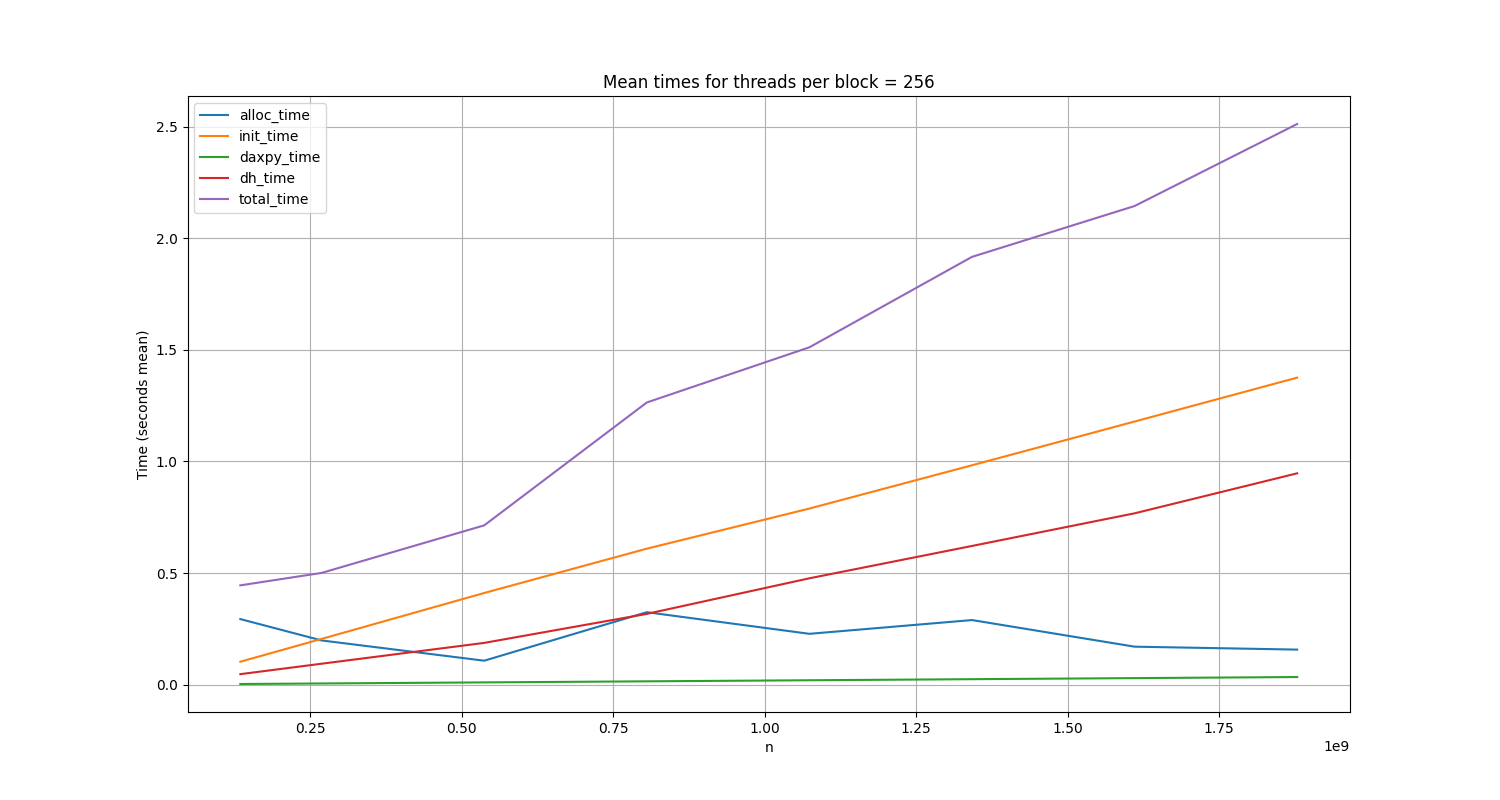
\includegraphics[width=0.9\textwidth]{images/daxpy/mean_times_256.png}
            }
            \caption{Mediciones de tiempo obtenidas para diferentes tamaños de problema.}
            \label{fig:daxpy_mean_times_256}
        \end{figure}        

        Un análisis pormenorizado de los componentes temporales revela características fundamentales del comportamiento de la implementación:
        
        \begin{itemize}
        
            \item El tiempo de inicialización (\texttt{init\_time}) domina el rendimiento global para problemas de gran magnitud, incrementando desde aproximadamente 0.1 segundos hasta 1.4 segundos a medida que aumenta el tamaño del problema. Este comportamiento se atribuye a la función \textit{kernel} \texttt{init\textless\textless\textless blocksPerGrid, threadsPerBlock\textgreater\textgreater\textgreater} que debe inicializar cada elemento de los vectores \texttt{x} e \texttt{y}. La clara progresión lineal confirma que la inicialización está limitada principalmente por el ancho de banda de memoria, no por la capacidad computacional intrínseca de la GPU.
            
            \item El tiempo de transferencia de datos hacia el host (\texttt{dh\_time}), implementado mediante \texttt{cudaMemPrefetchAsync}, exhibe asimismo un incremento lineal conforme aumenta el tamaño del problema. Este comportamiento es coherente con las expectativas teóricas, dado que el volumen de datos transferidos es directamente proporcional a $n$. La pendiente menos pronunciada en comparación con \texttt{init\_time} sugiere un aprovechamiento más eficiente del ancho de banda PCIe durante la transferencia unidireccional.
        
            \item El tiempo de asignación de memoria (\texttt{alloc\_time}) presenta un comportamiento particularmente interesante: inicialmente aumenta con el tamaño del problema hasta aproximadamente $n \approx 0.75 \times 10^9$, pero posteriormente se estabiliza e incluso manifiesta una ligera disminución. Este patrón no monotónico podría atribuirse a mecanismos internos de optimización en la gestión de memoria unificada de CUDA, como la asignación bajo demanda o la reserva anticipada de grandes bloques contiguos de memoria.
        
            \item El tiempo de ejecución específico del \textit{kernel} DAXPY (\texttt{daxpy\_time}) permanece notablemente constante y reducido (cercano a 0.05 segundos) independientemente del tamaño del problema. Este excepcional rendimiento se atribuye a dos factores fundamentales en la implementación:
        
                \begin{enumerate}
                
                    \item La utilización de un patrón de acceso con \textit{stride} en el \textit{kernel}. Esta estrategia permite que cada hilo procese múltiples elementos no contiguos, distribuyendo eficientemente la carga computacional incluso cuando el tamaño del problema excede significativamente el número total de hilos disponibles.
                    
                    \item La elevada intensidad aritmética característica de la operación DAXPY, combinada con un patrón de acceso a memoria perfectamente coalescente, maximiza la utilización efectiva del ancho de banda de memoria disponible en la GPU.
                    
                \end{enumerate}

        \end{itemize}
        
        La escalabilidad observada corrobora que la implementación está limitada principalmente por operaciones intensivas en memoria (inicialización y transferencia de datos), no por capacidad computacional, lo cual es característico de algoritmos clasificados como \textit{memory-bound}, como DAXPY, que presentan una relación operaciones aritméticas/accesos a memoria extremadamente baja.
        
    \subsection{Tiempo de ejecución}

        La figura \ref{fig:daxpy_times_per_threadsPerBlock} desglosa los tiempos de ejecución según la configuración de hilos por bloque, revelando patrones críticos para la optimización del rendimiento:

        \begin{figure}[H]
            \centering
            \fbox{
                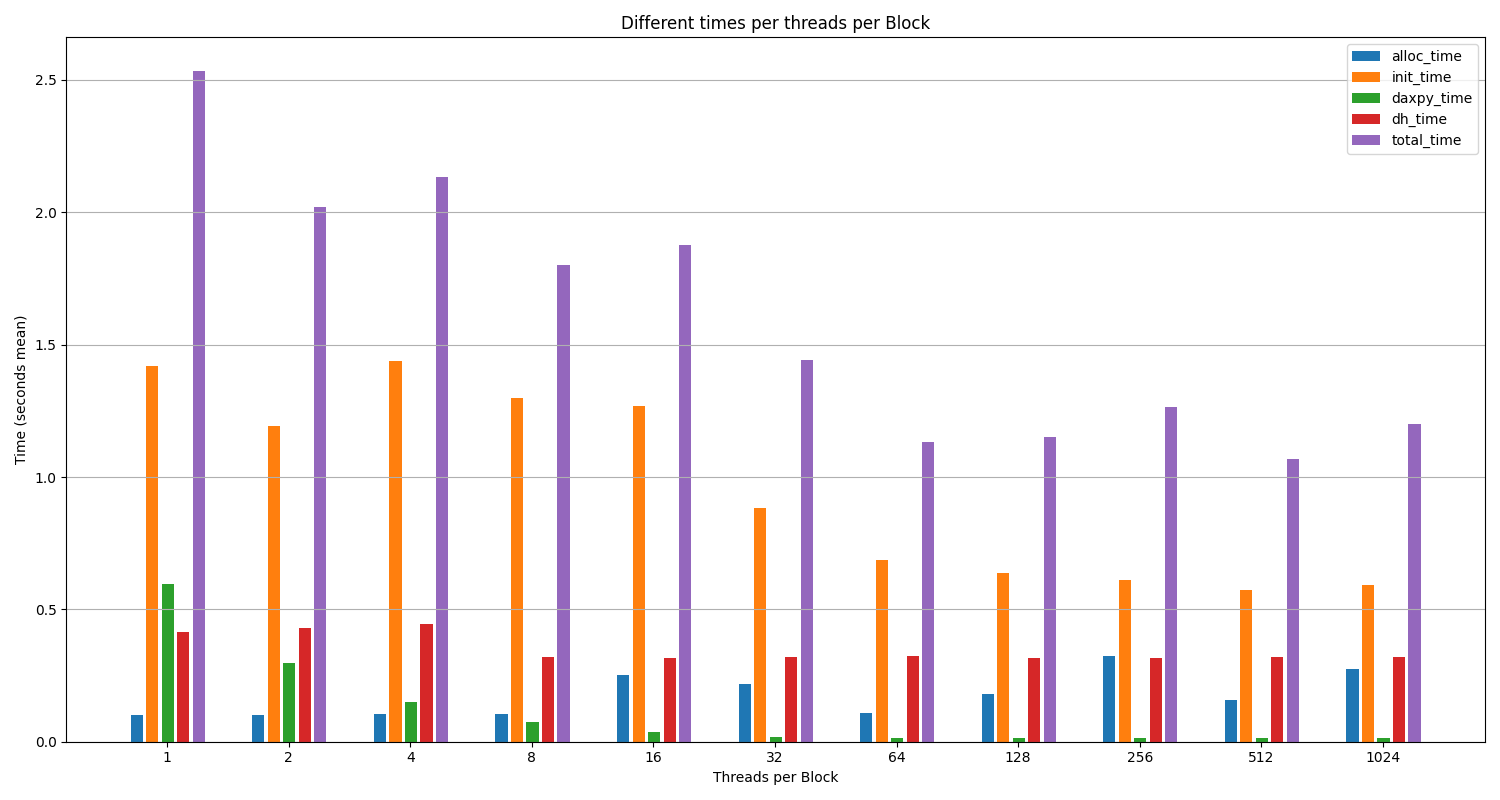
\includegraphics[width=0.9\textwidth]{images/daxpy/times_per_threadsPerBlock.png}
            }
            \caption{Mediciones de tiempo obtenidas para diferentes tamaños de bloques y \textit{grid}.}
            \label{fig:daxpy_times_per_threadsPerBlock}
        \end{figure}  
        
        \begin{itemize}
        
            \item Para configuraciones con baja densidad de hilos por bloque (1-4), el tiempo total de ejecución resulta excesivamente elevado (2.5 segundos para la configuración de 1 hilo por bloque). Este deficiente rendimiento se atribuye fundamentalmente a la incapacidad intrínseca de ocultar latencias de acceso a memoria y a la severa subutilización de los recursos computacionales disponibles en la GPU. Con tan escasa cantidad de hilos, la mayoría de los CUDA \textit{cores} permanecen en estado de inactividad, y el \textit{warp scheduler }no logra aprovechar eficientemente el paralelismo a nivel de \textit{warp} para mitigar las latencias de memoria.
            
            \item El tiempo de inicialización (\texttt{init\_time}) exhibe una pronunciada disminución al incrementar el número de hilos por bloque hasta aproximadamente 32 hilos, para luego continuar decreciendo más gradualmente. Este comportamiento se alinea perfectamente con la arquitectura de \textit{warps} característica de NVIDIA, donde cada \textit{warp} consta de exactamente 32 hilos ejecutándose en \textit{lockstep}. Las configuraciones por debajo de 32 hilos subutilizan inherentemente los recursos del \textit{warp} y generan un \textit{scheduling} ineficiente.
            
            \item El tiempo de ejecución específico del \textit{kernel} DAXPY (\texttt{daxpy\_time}) muestra una tendencia particularmente reveladora: es significativamente elevado (0.6 segundos) para la configuración de 1 hilo por bloque y disminuye rápidamente, tornándose prácticamente insignificante para configuraciones con más de 16 hilos por bloque. Esto evidencia la extraordinaria efectividad del paralelismo en la ocultación de latencias de memoria cuando se utiliza una cantidad suficiente de hilos, permitiendo que el \textit{kernel} opere a velocidades próximas al límite teórico impuesto por el ancho de banda de memoria.
            
            \item El punto óptimo de configuración se sitúa en torno a 128-256 hilos por bloque, donde el tiempo total alcanza su mínimo. Configuraciones con mayor densidad de hilos (512, 1024) no ofrecen mejoras adicionales significativas, lo que sugiere que otros factores limitantes, como la presión sobre los registros disponibles o la memoria compartida, podrían estar estableciendo un límite superior al rendimiento alcanzable.
        
        \end{itemize}
               
        El patrón de acceso implementado, conocido como ``grid-stride loop'', permite que la implementación escale eficientemente independientemente de la relación entre el tamaño del problema y el número total de hilos disponibles. Cuando se dispone de una cantidad insuficiente de hilos, cada hilo debe procesar secuencialmente numerosos elementos, lo que explica el deficiente rendimiento observado con configuraciones de baja densidad de hilos por bloque. Al incrementar el número de hilos, la carga computacional por hilo disminuye significativamente, mejorando la capacidad de ocultación de latencias y optimizando la utilización global de los recursos.
        
    \subsection{Ocupancia}

        La figura \ref{fig:daxpy_occupancy_per_threadsPerBlock} ilustra con precisión cómo la ocupancia teórica de los multiprocesadores de la GPU (SM) varía en función del número de hilos por bloque, proporcionando \textit{insights} fundamentales sobre la utilización de recursos:

        \begin{figure}[H]
            \centering
            \fbox{
                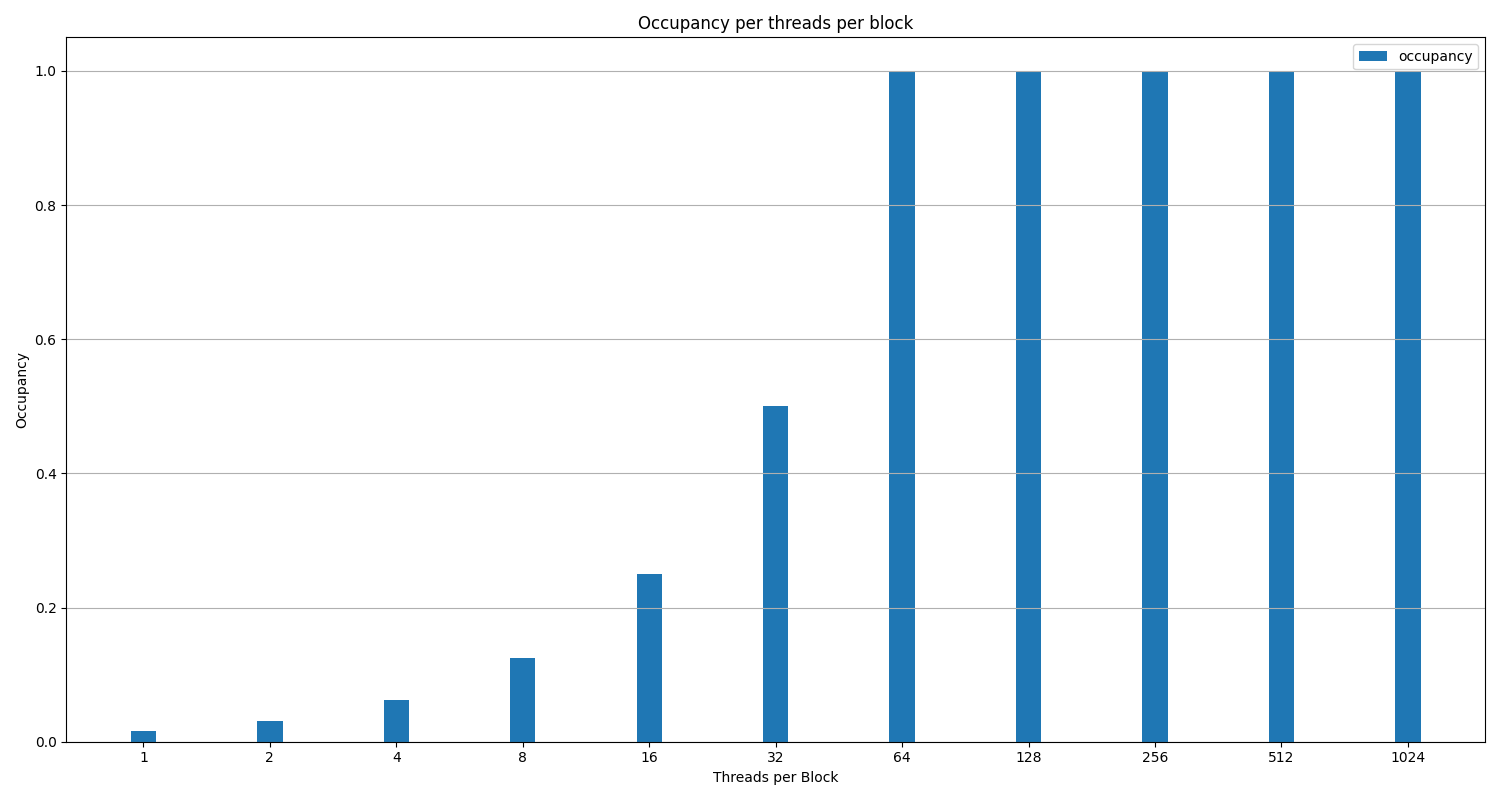
\includegraphics[width=0.9\textwidth]{images/daxpy/occupancy_per_threadsPerBlock.png}
            }
            \caption{Valores de ocupancia teorica para distintos valores de tamaño de bloque.}
            \label{fig:daxpy_occupancy_per_threadsPerBlock}
        \end{figure}  
        
        \begin{itemize}
        
            \item Para configuraciones con baja densidad de hilos por bloque (1-32), la ocupancia se mantiene en niveles extremadamente reducidos (inferior a 0.5), lo que explica satisfactoriamente el deficiente rendimiento observado en estas configuraciones. Cuando la ocupancia es baja, el \textit{hardware} no puede implementar eficazmente mecanismos para ocultar latencias de acceso a memoria mediante el cambio de contexto entre \textit{warps}, resultando en una ejecución notablemente ineficiente.
            
            \item Un punto de inflexión crítico se observa en la configuración de 64 hilos por bloque, donde la ocupancia alcanza súbitamente el valor máximo de 1.0 (100\%). Esta ocupancia óptima se mantiene constante para todas las configuraciones de mayor densidad (128, 256, 512, 1024 hilos por bloque). Este comportamiento se relaciona directamente con los algoritmos de cálculo de ocupancia implementados en el código. La ocupancia perfecta indica que la GPU logra mantener suficientes bloques activos por SM para saturar completamente sus recursos de ejecución, lo que teóricamente debería traducirse en un rendimiento óptimo.
            
            \item Resulta particularmente significativo observar que, a pesar de alcanzar una ocupancia perfecta a partir de 64 hilos por bloque, el rendimiento óptimo (figura 1) se manifiesta con configuraciones de 128-256 hilos por bloque. Esta aparente discrepancia revela que la ocupancia teórica no constituye el único factor determinante del rendimiento práctico. Otros factores críticos como el tamaño del \textit{working} set en las cachés L1/L2, la eficiencia en la coalescencia de accesos a memoria, y la potencial divergencia de \textit{warps} desempeñan roles igualmente importantes en la determinación del rendimiento global.
        
        \end{itemize}
        
        La ocupancia está influenciada principalmente por tres limitaciones fundamentales de recursos: el número de registros disponibles por hilo, la cantidad de memoria compartida por bloque y el número máximo de hilos que pueden residir simultáneamente en cada SM. En este caso particular, dado que el \textit{kernel} DAXPY presenta una estructura relativamente simple y utiliza una cantidad reducida de registros sin requerir memoria compartida, el factor limitante predominante es probablemente el número máximo de \textit{threads} que pueden coexistir simultáneamente en cada SM. A partir de cierto umbral (64 hilos por bloque), el \textit{hardware} logra programar eficientemente suficientes \textit{warps} para mantener todos los CUDA \textit{cores} en estado de ocupación incluso cuando algunos \textit{warps} se encuentran en espera por operaciones de memoria.

    \subsection{Matriz de isoeficiencia}

        La figura \ref{fig:daxpy_isoEfficiencyMatrix} presenta una matriz de isoeficiencia que proporciona una visión holística y multidimensional del rendimiento en función de dos variables críticas: el tamaño del problema (eje horizontal) y el número de hilos por bloque (eje vertical). Esta sofisticada visualización permite identificar regiones de eficiencia comparable a través de diversas configuraciones.

        \begin{figure}[H]
            \centering
            \fbox{
                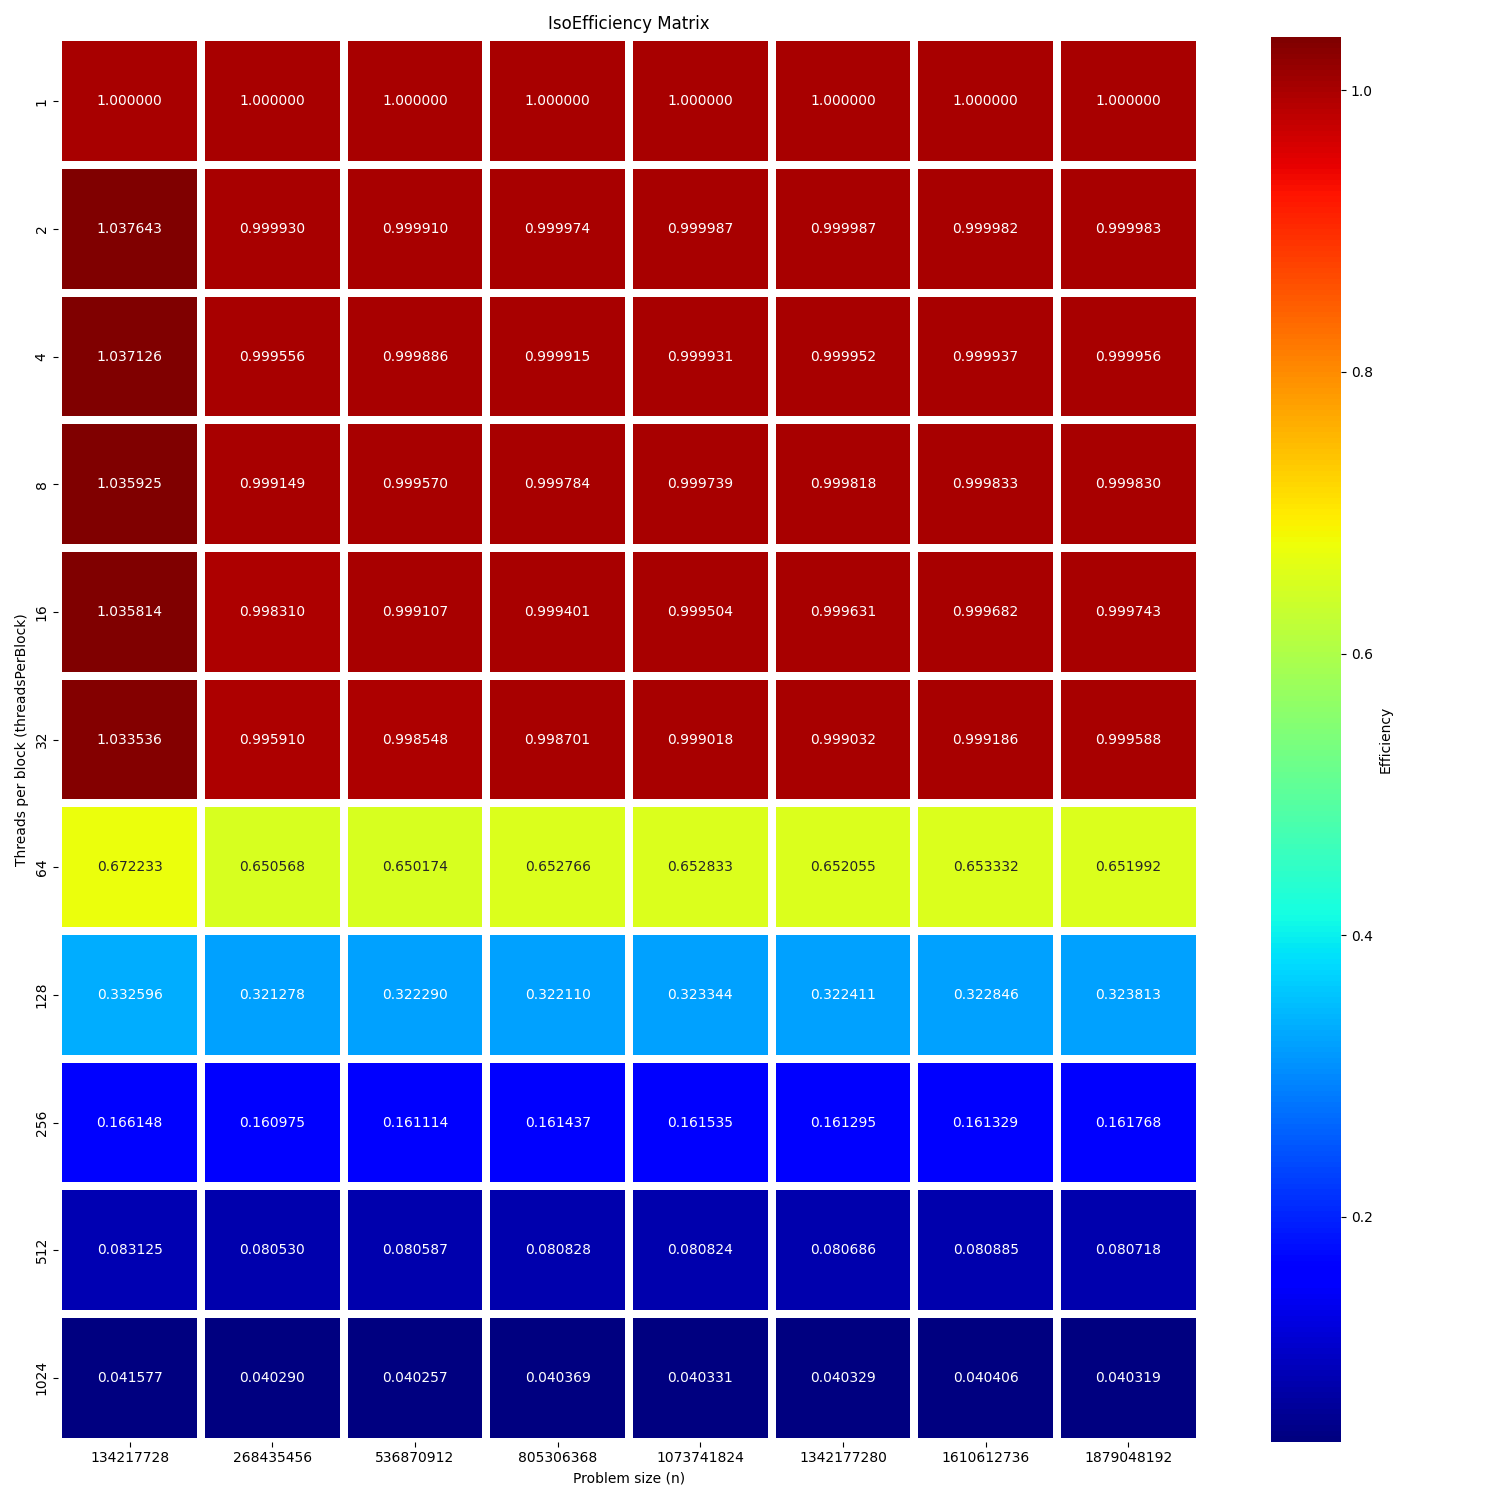
\includegraphics[width=0.9\textwidth]{images/daxpy/isoEfficiencyMatrix.png}
            }
            \caption{Matriz de isoeficiencia.}
            \label{fig:daxpy_isoEfficiencyMatrix}
        \end{figure}  
        
        \begin{itemize}
        
            \item Las configuraciones con baja densidad de hilos por bloque (1-32) exhiben una eficiencia aparentemente elevada (valores cercanos a 1.0), representada mediante tonalidades rojizas en la región superior de la matriz. Sin embargo, esta elevada eficiencia resulta engañosa cuando se analiza en conjunción con los resultados de tiempo de ejecución y ocupancia. Estas configuraciones son ``eficientes'' únicamente en el sentido de que mantienen una relación relativamente constante entre rendimiento y recursos utilizados, pero su rendimiento absoluto es marcadamente deficiente debido a la insuficiente utilización de los recursos computacionales disponibles en la GPU.
        
            \item Se observa una transición dramática en la eficiencia precisamente en la configuración de 64 hilos por bloque, donde los valores experimentan una súbita reducción hasta aproximadamente 0.67 (representada mediante tonalidades amarillentas). Esta transición crítica coincide exactamente con el punto donde la ocupancia alcanza su valor máximo de 1.0, lo que sugiere convincentemente que a partir de este umbral la implementación está limitada fundamentalmente por el ancho de banda de memoria disponible, no por la capacidad computacional intrínseca.
            
            \item Las configuraciones con alta densidad de hilos por bloque (128 o superior) muestran una eficiencia progresivamente decreciente (tonalidades azuladas), con valores que descienden hasta aproximadamente 0.04 para la configuración máxima de 1024 hilos por bloque. Esta disminución no debe interpretarse necesariamente como un deterioro del rendimiento absoluto, sino como una indicación de que estas configuraciones no escalan linealmente con el incremento de recursos asignados.
            
            \item Resulta particularmente notable que la eficiencia se mantiene notablemente constante a través de diferentes tamaños de problema para una configuración dada de hilos por bloque, como se evidencia por la uniformidad cromática en cada fila horizontal de la matriz. Esta observación corrobora que el rendimiento está determinado principalmente por el grado de paralelismo implementado (hilos por bloque) y no por el tamaño específico del problema, una vez que éste supera cierto umbral crítico.
            
        \end{itemize}
        
        La interpretación comprehensiva de esta matriz debe realizarse necesariamente en conjunción con las restantes métricas analizadas. Por ejemplo, aunque las configuraciones con baja densidad de hilos por bloque exhiben una elevada ``eficiencia'' aparente, sabemos por los análisis de ocupancia y tiempo de ejecución (Figuras 2 y 1, respectivamente) que su rendimiento absoluto es notablemente deficiente debido a la insuficiente ocupancia. La matriz resalta claramente que, para este algoritmo clasificado como \textit{memory-bound}, existe un punto óptimo en torno a 64-128 hilos por bloque que establece un equilibrio adecuado entre ocupancia efectiva y otros factores limitantes como la presión sobre los registros disponibles y las cachés.

        Esta sofisticada visualización refleja asimismo una característica fundamental de los algoritmos \textit{ memory-bound} como DAXPY: una vez que se alcanza un nivel suficiente de paralelismo para saturar completamente el ancho de banda de memoria disponible, la incorporación de paralelismo adicional no contribuye significativamente a la mejora del rendimiento, resultando en una eficiencia aparentemente reducida, pero manteniendo un rendimiento absoluto óptimo desde la perspectiva práctica.

    \subsection{Métricas generales}

        \begin{table}[H]
            \centering
            \begin{adjustbox}{width=\textwidth, keepaspectratio}
                \begin{tabular}{rrrrrrrrr}
                    \toprule
                    Threads & N & Max Time & Ref Time & Speedup & Efficiency & Quality & Secuential Compute Speedup & Secuential Total Speedup \\
                    \midrule
                    16 & 134217728 & 0.01 & 0.10 & 16.57 & 1.04 & 160.57 & 136.71 & 11.46 \\
                    32 & 134217728 & 0.00 & 0.10 & 33.07 & 1.03 & 320.43 & 272.81 & 5.59 \\
                    64 & 134217728 & 0.00 & 0.10 & 43.02 & 0.67 & 416.83 & 354.89 & 5.84 \\
                    128 & 134217728 & 0.00 & 0.10 & 42.57 & 0.33 & 412.46 & 351.17 & 5.95 \\
                    256 & 134217728 & 0.00 & 0.10 & 42.53 & 0.17 & 412.09 & 350.85 & 5.91 \\
                    512 & 134217728 & 0.00 & 0.10 & 42.56 & 0.08 & 412.34 & 351.07 & 5.52 \\
                    1024 & 134217728 & 0.00 & 0.10 & 42.58 & 0.04 & 412.49 & 351.19 & 5.99 \\
                    
                    16 & 268435456 & 0.01 & 0.20 & 15.97 & 1.00 & 80.32 & 68.39 & 4.89 \\
                    32 & 268435456 & 0.01 & 0.20 & 31.87 & 1.00 & 160.26 & 136.45 & 4.39 \\
                    64 & 268435456 & 0.00 & 0.20 & 41.64 & 0.65 & 209.38 & 178.26 & 4.79 \\
                    128 & 268435456 & 0.00 & 0.20 & 41.12 & 0.32 & 206.80 & 176.07 & 4.85 \\
                    256 & 268435456 & 0.00 & 0.20 & 41.21 & 0.16 & 207.23 & 176.44 & 4.92 \\
                    512 & 268435456 & 0.00 & 0.20 & 41.23 & 0.08 & 207.34 & 176.53 & 5.00 \\
                    1024 & 268435456 & 0.00 & 0.20 & 41.26 & 0.04 & 207.47 & 176.64 & 5.02 \\

                    16 & 536870912 & 0.02 & 0.40 & 15.99 & 1.00 & 40.20 & 34.22 & 2.29 \\
                    32 & 536870912 & 0.01 & 0.40 & 31.95 & 1.00 & 80.35 & 68.41 & 3.15 \\
                    64 & 536870912 & 0.01 & 0.40 & 41.61 & 0.65 & 104.63 & 89.08 & 5.58 \\
                    128 & 536870912 & 0.01 & 0.40 & 41.25 & 0.32 & 103.73 & 88.32 & 5.76 \\
                    256 & 536870912 & 0.01 & 0.40 & 41.25 & 0.16 & 103.71 & 88.30 & 5.98 \\
                    512 & 536870912 & 0.01 & 0.40 & 41.26 & 0.08 & 103.75 & 88.33 & 6.08 \\
                    1024 & 536870912 & 0.01 & 0.40 & 41.22 & 0.04 & 103.65 & 88.25 & 5.98 \\
                   
                    16 & 805306368 & 0.04 & 0.60 & 15.99 & 1.00 & 26.81 & 22.82 & 1.88 \\
                    32 & 805306368 & 0.02 & 0.60 & 31.96 & 1.00 & 53.57 & 45.61 & 2.30 \\
                    64 & 805306368 & 0.01 & 0.60 & 41.78 & 0.65 & 70.03 & 59.63 & 3.79 \\
                    128 & 805306368 & 0.01 & 0.60 & 41.23 & 0.32 & 69.11 & 58.84 & 3.27 \\
                    256 & 805306368 & 0.01 & 0.60 & 41.33 & 0.16 & 69.28 & 58.98 & 3.32 \\
                    512 & 805306368 & 0.01 & 0.60 & 41.38 & 0.08 & 69.37 & 59.06 & 3.37 \\
                    1024 & 805306368 & 0.01 & 0.60 & 41.34 & 0.04 & 69.30 & 59.00 & 3.37 \\
                   
                    16 & 1073741824 & 0.05 & 0.80 & 15.99 & 1.00 & 20.11 & 17.12 & 1.66 \\
                    32 & 1073741824 & 0.02 & 0.80 & 31.97 & 1.00 & 40.19 & 34.22 & 1.86 \\
                    64 & 1073741824 & 0.02 & 0.80 & 41.78 & 0.65 & 52.53 & 44.72 & 2.31 \\
                    128 & 1073741824 & 0.02 & 0.80 & 41.39 & 0.32 & 52.03 & 44.30 & 2.44 \\
                    256 & 1073741824 & 0.02 & 0.80 & 41.35 & 0.16 & 51.99 & 44.26 & 2.49 \\
                    512 & 1073741824 & 0.02 & 0.80 & 41.38 & 0.08 & 52.03 & 44.30 & 2.48 \\
                    1024 & 1073741824 & 0.02 & 0.80 & 41.30 & 0.04 & 51.92 & 44.21 & 2.49 \\
                    
                    16 & 1342177280 & 0.06 & 0.99 & 15.99 & 1.00 & 16.09 & 13.70 & 1.40 \\
                    32 & 1342177280 & 0.03 & 0.99 & 31.97 & 1.00 & 32.15 & 27.38 & 1.70 \\
                    64 & 1342177280 & 0.02 & 0.99 & 41.73 & 0.65 & 41.97 & 35.74 & 2.07 \\
                    128 & 1342177280 & 0.02 & 0.99 & 41.27 & 0.32 & 41.51 & 35.34 & 1.82 \\
                    256 & 1342177280 & 0.02 & 0.99 & 41.29 & 0.16 & 41.53 & 35.36 & 1.88 \\
                    512 & 1342177280 & 0.02 & 0.99 & 41.31 & 0.08 & 41.55 & 35.38 & 1.90 \\
                    1024 & 1342177280 & 0.02 & 0.99 & 41.30 & 0.04 & 41.54 & 35.36 & 1.87 \\
                    
                    16 & 1610612736 & 0.07 & 1.19 & 15.99 & 1.00 & 13.41 & 11.41 & 1.27 \\
                    32 & 1610612736 & 0.04 & 1.19 & 31.97 & 1.00 & 26.80 & 22.82 & 1.59 \\
                    64 & 1610612736 & 0.03 & 1.19 & 41.81 & 0.65 & 35.05 & 29.84 & 1.93 \\
                    128 & 1610612736 & 0.03 & 1.19 & 41.32 & 0.32 & 34.64 & 29.49 & 1.60 \\
                    256 & 1610612736 & 0.03 & 1.19 & 41.30 & 0.16 & 34.62 & 29.47 & 1.64 \\
                    512 & 1610612736 & 0.03 & 1.19 & 41.41 & 0.08 & 34.71 & 29.55 & 1.65 \\
                    1024 & 1610612736 & 0.03 & 1.19 & 41.38 & 0.04 & 34.68 & 29.53 & 1.61 \\
                   
                    16 & 1879048192 & 0.09 & 1.39 & 16.00 & 1.00 & 11.49 & 9.78 & 1.05 \\
                    32 & 1879048192 & 0.04 & 1.39 & 31.99 & 1.00 & 22.98 & 19.57 & 1.36 \\
                    64 & 1879048192 & 0.03 & 1.39 & 41.73 & 0.65 & 29.98 & 25.52 & 1.50 \\
                    128 & 1879048192 & 0.03 & 1.39 & 41.45 & 0.32 & 29.78 & 25.35 & 1.44 \\
                    256 & 1879048192 & 0.03 & 1.39 & 41.41 & 0.16 & 29.75 & 25.33 & 1.59 \\
                    512 & 1879048192 & 0.03 & 1.39 & 41.33 & 0.08 & 29.69 & 25.28 & 1.61 \\
                    1024 & 1879048192 & 0.03 & 1.39 & 41.29 & 0.04 & 29.66 & 25.25 & 1.58 \\
                    \bottomrule
                \end{tabular}
            \end{adjustbox}
            \caption{Métricas generales.}
            \label{tab:daxpy_metrics}
        \end{table}  
